\section{Felder (arrays) und Zeichenketten}

Bisher haben wir uns ausschließlich mit skalaren Datentypen beschäftigt, d.h. also einzelne Elemente eines bestimmten Typs.
\texttt{C} kennt allerdings auch Tupel eines bestimmten Typs, sogenannte Felder oder im Englischen \emph{arrays}.
Allerdings muss die Länge des Tupels zum Zeitpunkt der Deklaration bekannt sein.
Und diese Länge kann auch dann nicht mehr verändert werden.

\subsection{Deklaration und Initialisierung eindimensionaler Felder}

Die Deklaration eines Feldes ist ganz analog zu anderen Variablen
\begin{lstlisting}
  int a[5]; // array declaration
\end{lstlisting}
was in diesem Fall ein Feld der Länge $5$ mit ganzen Zahlen erzeugt.

Für die Initialisierung gibt es zwei Möglichkeiten.
Man kann erstens Deklaration und Initialisierung in einem Schritt vornehmen
\begin{lstlisting}
  int a1[5] = {1, 2, 3, 4, 5};
  int a2[] = {1, 2, 3, 4, 5};
\end{lstlisting}
was jeweils ein Feld der Länge $5$ erzeugt, aber diesmal initialisiert mit den Werten $1,2,3,4,5$.
Bei der zweiten Zeile bestimmt der Compiler aus der Initialisierungsliste automatisch die Länge des Feldes.
Die zweite Möglichkeit besteht darin, jedes Element einzeln zuzuweisen:
\begin{lstlisting}
  int a[5];
  for(int i = 0; i < 5; i++) {
    a[i] = i+1;
  }
\end{lstlisting}
was zum exakt gleichen Ergebnis führt.
An diesem Beispiel sieht man bereits, dass in \texttt{C} die Indizierung von $0$ bis $n-1$ läuft.
Außerdem kann auf die einzelnen Elemente des Feldes mit dem Indexoperator \verb|[ ]| zugegriffen werden.
Erlaubte Argumente für den Indexoperator \verb|[ ]| sind positive ganze Zahlen.\index{Indexoperator \texttt{[ ]}}\index{\texttt{[ ]}}

Es sei nocheinmal darauf hingewiesen, dass Felder wie wir sie bisher eingeführt haben, konstante Länge haben.
So führt folgender Quelltext zu einer Fehlermeldung
\begin{lstlisting}
  int n = 5;
  int a[n];
\end{lstlisting}
da die Variable \texttt{n} nicht konstant ist.
Dagegen ist folgendes korrekt
\begin{lstlisting}
  const int n = 5;
  int a[n];
  for(int i = 0; i < n; i++) {
    a[i] = i+1;
  }
\end{lstlisting}
was es erlaubt die Feldlänge in einer Variablen zu speichern.
Wenn sich nun im Quelltext diese Länge ändert, so muss man diese Änderung nur noch an einer Stelle vornehmen.


\subsection{Eindimensionale Felder als Funktionenargumente}

Wie schon im Abschnitt über Funktionen angedeutet, kann man auch Felder als Funktionenargument verwenden.
Die Schreibweise wird am folgenden Beispiel für eine Funktion erklärt, die die Quadratsumme aller Elemente eines Feldes erzeugt (das Quadrat der Norm)
\begin{lstlisting}
  double sqrsum(double a[], const int n) {
    double sum = 0;
    for(int i = 0; i < n; i++) {
      sum += a[i]*a[i];
    }
    return sum;
  }
\end{lstlisting}
Die Schreibweise \texttt{a[]} teilt dem Compiler mit, dass es sich um ein Feld handelt.
Es ist sehr wichtig hier zu verstehen, dass der Compiler aber keine Möglichkeit hat zu überprüfen, ob innerhalb der Funktion nur auf die vorhandenen Elemente von \texttt{a} zugegriffen wird.
Man muss als Programmierer also darauf achten, dass diese Information verfügbar gemacht wird und nicht verlorengeht.
In diesem Fall bedeutet das, dass \texttt{n} die richtige Länge als Wert enthalten muss.
Folgender Quelltext ist korrekter \texttt{C} Quelltext
\begin{lstlisting}
int list[5];
int i = 5;
list[i] = 3;
\end{lstlisting}
und wird vom Compiler anstandslos übersetzt.
Im besten Fall erhält man dann bei der Ausführung dieses Codes einen \emph{segmentation fault}.
Im schlechtesten Fall ist \verb|list[5]| Speicher, auf den das Programm zugreifen kann.
Dann erhält man keinen Laufzeitfehler und modifiziert ungewollt Speicher, den man nicht modifizieren will.
Dies kann zu sehr seltsamem Verhalten des Programms führen, und das Finden eines solchen Fehlers ist sehr schwierig.
Deshalb sollte man Indizierungen immer mit großer Sorgfalt überprüfen.

Es gibt noch einen weiteren wichtigen Punkt, der später noch genauer diskutiert wird.
Für Felder, die man wie oben beschrieben an Funktionen übergibt, wird keine Kopie angelegt.
Das heißt insbesondere, dass sich das Originalfeld ändert, wenn man innerhalb der Funktion das Feld modifiziert.
Genauer wird das im Abschnitt über Zeiger diskutiert.

\subsection{Mehrdimensionale Felder}

Ganz analog zu eindimensionalen Feldern lassen sich auch zweidimensionale Felder (Matrizen) erzeugen
\begin{lstlisting}
  int A[3][5]; // Deklaration
  for(int i = 0; i < 3; i++) {
    for(int j = 0; j < 5; j++) {
      A[i][j] = i+j;  // Initialisierung
    }
  }
\end{lstlisting}
Und wie im eindimensionalen Fall kann man auch Deklaration und Initialisierung kombinieren
\begin{lstlisting}
  int A1[3][3] = {{1,2,3}, {4,5,6}, {7,8,9}};
  int A2[][3]  = {{1,2,3}, {4,5,6}, {7,8,9}};
  int A3[][3] = {1,2,3,4,5,6,7,8,9}};
\end{lstlisting}
Die Anzahl der Zeilen kann der Compiler aus der Initialisierungsliste bestimmen.
Die Anzahl der Spalten muss aber immer angegeben sein.
Die Dimensionalität eines Feldes kann dann in analoger Weise zu drei oder mehr erweitert werden, wobei der \texttt{C}-Compiler die Feldelemente immer linear so im Speicher ablegt, wie für das Beispiel \texttt{A1} in Abbildung~\ref{fig:2darray} gezeigt.
Das heißt, dass die Dimensionen des Arrays von rechts nach links zählend linear im Speicher abgelegt werden.

\begin{figure}[!ht]
  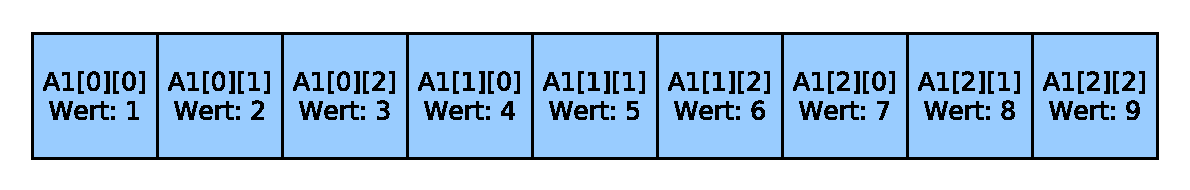
\includegraphics[width=\textwidth]{graphics/2darray_im_speicher}
  \caption{\label{fig:2darray} Das zweidimensionale Array \texttt{A1} im Speicher.}
\end{figure}

Die Benutzung von Feldern wird in folgendem Beispiel illustriert:
\begin{myexampleprogram}{Beispiel: Berechnung des Mittelwerts und der Varianz}
  Die Berechnung des Mittelwerts einer Datenreihe ist ein gutes Beispiel für die Benutzung von Arrays.
  Nehmen wir an, wir haben die folgenden Daten gegeben:
\begin{lstlisting}
double data[] = {1.3, 2.4, 5.3, 2.4, 6.7, 3.5, 6.9, 1.3, 1.4, 4.5,
                 5.5, 5.3, 6.7, 2.1, 2.4, 3.3, 7.9, 0.3, 3.3, 1.5};
\end{lstlisting}
  und wir wollen den Mittelwert dieser Daten berechnen.
  Folgendes Program übernimmt diese Aufgabe:
\begin{lstlisting}
#include <stdio.h>

int main()
{
  const int size = 20;
  double data[] = {1.3, 2.4, 5.3, 2.4, 6.7, 3.5, 6.9, 1.3, 1.4, 4.5,
                   5.5, 5.3, 6.7, 2.1, 2.4, 3.3, 7.9, 0.3, 3.3, 1.5};

  // initialisiere mean zu 0
  double mean = 0.;
  for (int i = 0; i < size; i++)
    {
      mean += data[i];
    }
  mean /= (double)size;
  printf("Der Mittelwert ist %e\n", mean);
  return (0);
}
\end{lstlisting}
  Für die Varianz müssen wir auch noch die Quadrate aufsummieren.
  Wir modifizieren dafür die Schleife wie folgt:
\begin{lstlisting}
double mean = 0., xsq = 0.;
for (int i = 0; i < size; i++)
  {
    mean += data[i];
    xsq += data[i] * data[i];
  }
mean /= (double)size;
\end{lstlisting}
  Die Varianz können wir dann wie folgt berechnen und ausgeben:
\begin{lstlisting}
double var = xsq / (double)size - mean * mean;
printf("Die Varianz ist %e\n", var);
\end{lstlisting}
\end{myexampleprogram}
\newpage

\subsection{Zeichenketten oder Strings}

In C gibt es keinen elementaren Datentyp für Zeichenketten, sogenannte \emph{strings}.
Zeichenketten werden mit Hilfe von Arrays abgebildet.
Ein Zeichen kann in einer Variablen vom Typ \verb|char| gespeichert werden.
Die Größe des Datentyps \texttt{char} ist immer ein Byte, also 8 Bit.\footnote{\textbf{Bemerkung:}~ Im ASCII Zeichensatz können $2^8= 256$ verschiedene Zeichen gespeichert werden.
Dies reicht für Englisch und ein paar Steuerzeichen, jedoch nicht für alle Sprachen dieser Welt.
Der ASCII Zeichensatz nutzt die ersten 128 Zustände (also die ersten 7 Bit) für das im Englischen genutzte Alphabet.
Die restlichen 128 Zustände werden abhängig vom  \emph{Encoding} interpretiert.
Für Deutsch kann man \texttt{latin-1} nutzen.
Je nach Encoding wird, z.B., ein Zeichen mit Wert 204 als solches oder jenes interpretiert.
Ist das Encoding nicht das richtige, erscheinen z.B. Zeichen mit Umlauten
nicht korrekt und scheinbar willkürliche Zeichen stehen an ihrer Stelle.
Sprachen, die mehr als 128 verschiedene Zeichen benötigen, können im oberen
Teil von ASCII überhaupt nicht dargestellt werden. Die Einsicht, dass es
mehr als 256 verschiedene Zeichen gibt, wurde im Unicode Standard
manifestiert. Die Konsequenz ist jedoch, dass jetzt mehr als ein Byte pro
Zeichen benötigt wird. UTF-8 ist inzwischen vielerorts das Standard-Encoding, sodass
beliebig viele verschiedene Zeichen in einer Textdatei genutzt werden
können. Der Preis ist jedoch, dass ein Buchstabe jetzt beliebig viele Byte
(meist eins) nutzt. Da hier der Fokus allerdings auf Numerischen Methoden
liegt, wird nicht weiter auf die vielfältigen Probleme mit Encodings
eingegangen.}

Eine Zeichenkette kann also durch eine Array von Elementen vom Typ \verb|char| erzeugt werden.
Das Ende einer Zeichenkette wird durch das Zeichen \verb|\0| angegeben.
Man spricht auch von \emph{null-terminiert} oder \emph{0-terminiert} und das Zeichen \verb|\0| wird auch \emph{Nullterminierungszeichen} genannt.
Im nächsten Beispiel überprüfen wir, ob eine Zeichenkette eine Zahl enthält:
\begin{myexampleprogram}{Beispiel: Durchsuchen von Zeichenketten}
\begin{lstlisting}
#include <stdio.h>

int main()
{
  char string[] = "sdfk99225kljsdfs\0";
  int i = 0;
  int ergebnis = 0;

  while(1) {
    if(string[i] == '\0') {
      break;
    }
    if((string[i]) >= '0' && (string[i] <= '9')) {
      ergebnis = 1;
      break;
    }
    i++;
  }
  if (ergebnis){
    printf("Der String %s enthaelt mindestens eine Zahl\n", string);
  } else {
    printf("Der String %s enthaelt keine Zahlen\n", string);
  }
  return 0;
}
\end{lstlisting}
\end{myexampleprogram}
Wir deklarieren und initialisieren zunächst die Variable \texttt{string} mit einer Zeichenkette.
Dann nutzen wir eine \verb|while| Schleife mit konstant wahrem logischem Ausdruck.
Die Schleife wird dann mit \verb|break| abgebrochen, wenn das Endstring-Zeichen gefunden wurde.
In der Schleife wird dann jedes Element der Kette darauf überprüft, ob es eine Zahl ist.
Dementsprechend wird die Variable \verb|ergebnis| gesetzt.
% BaKo: hier m.E. keine gute Stelle, um darauf hinzuweisen
%       erstens sind Strings speziell (weil terminiert)
%       zweitens sind die *printf Funktionen schrecklich kompliziert...
% Beim abschließenden \texttt{printf} wird eine wichtige Eigenschaft von \texttt{C} Feldern deutlich:
% Man benötigt keine Referenzierungsoperator \verb|&|.\index{Adressoperator \&}\index{\&}
% Im nächsten Abschnitt über Zeiger wird klar werden, warum dies so ist.

\subsubsection{Formatierte Erstellung von Zeichenketten mit \texttt{sprintf} und \texttt{snprintf}}

Die Manipulation von Zeichenketten ist oft ein wichtiger Bestandteil eines Programms, zum Beispiel um Ausgabedateinamen abhängig vom Wert einer Variable zu machen.

Wie haben die Funktion \texttt{printf} schon öfter zur Textausgabe verwendet und werden im Detail in Teil~\ref{sec:ein_ausgabe} auf die \emph{formatierte} Ausgabe eingehen.
Möchte man jedoch formatierte Textdarstellungen von Variablen nicht auf die Konsole, sondern direkt in eine Zeichenkette ausgeben, so stehen in \texttt{C} die beiden Funktionen \texttt{sprintf} und \texttt{snprintf} zur Verfügung.
Diese ähneln in ihrer Benutzung der bekannten \texttt{printf} Funktion und werden mit der Headerdatei \texttt{stdio.h} eingebunden.\index{\texttt{sprintf}}\index{\texttt{snprintf}}
Im Gegensatz zu \texttt{printf}, schreiben diese Funktionen jedoch direkt in eine sich im Speicher befindliche Zeichenkette.

Diese Funktionen haben die Signaturen
\begin{lstlisting}
  int sprintf(char *str, const char *format, ...);
  int snprintf(char *str, size_t size, const char *format, ...);
\end{lstlisting}
wobei das Argument \enquote{\texttt{str}} für die Zeichenkette steht, in die geschrieben werden soll und \enquote{\texttt{format}} eine konstante Zeichenkette ist, in der wir beschreiben werden, wie dies zu erfolgen hat.
Die Bedeutung von \enquote{\texttt{char *}} und \enquote{\texttt{const char *}} wird in Teil~\ref{sec:zeiger} noch genau erklärt werden.
Die sogenannte \emph{variable Argumentenliste}, \enquote{\texttt{...}}, dient bei den Funktionen aus \texttt{stdio.h} als Platzhalter für eine beliebige Anzahl von Variablen oder Konstanten, die man ausgeben möchte.
Bei \texttt{snprintf} steht das Argument \enquote{\texttt{size}} für die maximale Anzahl an Zeichen (inklusive des Nullterminierungszeichens), welche in die Zeichenkette \texttt{str} geschrieben werden soll.
Die Stelle in der Zeichenkette, an denen diese Ausgabe stattfinden soll, sowie das Format in der diese Ausgabe erfolgen soll, geben wir anhand von Platzhaltern an, genau so, wie wir es auch schon bei \texttt{printf} getan haben.

Da wir jedoch nicht auf die Konsole ausgeben, sondern direkt in Speicher schreiben, muss man bei der Verwendung insbesondere von \texttt{sprintf} sehr vorsichtig sein, wie in folgendem Beispiel gezeigt wird.

\begin{myexampleprogram}{Beispiel: Formatierte Erstellung von Zeichenketten mit \texttt{sprintf} und \texttt{snprintf}}
\begin{lstlisting}[numbers=left]
#include <stdio.h>
// konstante Längen für lange und kurze Zeichenketten
const int MAX_LENGTH = 1000;
const int SHORT_LENGTH = 50;

int main()
{
  char string[MAX_LENGTH];
  const int i = 42;
  sprintf(string,
          "The Answer to the Ultimate Question of Life,"
          "The Universe, and Everything is %d.\n\n",
          i);
  printf("string: %s", string);
  
  int rval;
  char short_string[SHORT_LENGTH];
  
  // kurze Zeichenkette wird in short_string geschrieben
  // Rueckgaberwert wird ueberprueft
  rval = snprintf(short_string, 
                  SHORT_LENGTH-1, 
                  "This is a test string.\n\n");
  if(rval >= SHORT_LENGTH) {
    printf("snprintf: The string was not completely written!\n");
  } else {
    printf("snprintf: wrote %d characters\n", rval);
  }
  printf("short_string: %s",short_string);
  
  // ueberlange Zeichenkette wird in short_string geschrieben
  // Rueckgaberwert wird ueberprueft
  rval = snprintf(short_string, 
                  SHORT_LENGTH-1, 
                  "The Answer to the Ultimate Question of Life, "
                  "The Universe, and Everything is %d.\n", 
                  i);
                  
  if(rval >= SHORT_LENGTH) {
    printf("snprintf: The string was not completely written!\n");
  }
  
  printf("short_string: %s\n\n",short_string);
  
  // ACHTUNG: hier wird fremder Speicher ueberschrieben 
  sprintf(short_string, 
          "The Answer to the Ultimate Question of Life"
          ", The Universe, and Everything is %d.\n",
          i);
  printf("short_string: %s",short_string); 
  
  return 0;
}
\end{lstlisting}
\noindent \textbf{Ausgabe des Beispielprogramms:}
{\footnotesize
\begin{lstlisting}[numbers=left]
$ ./test
string: The Answer to the Ultimate Question of Life, The Universe, and Everything is 42.

snprintf: wrote 24 characters
short_string: This is a test string.

snprintf: The string was not completely written!
short_string: The Answer to the Ultimate Question of Life, The

short_string: The Answer to the Ultimate Question of Life, The Universe, and Everything is 42.
\end{lstlisting}
}

\end{myexampleprogram}
Ebenso wie bei \texttt{scanf}, besteht die Gefahr eines buffer overflows, wenn mit \texttt{sprintf} mehr Zeichen geschrieben werden, als eigentlich allokiert wurden.
Dies resultiert im schlimmsten Fall \emph{nicht} in einem Programmabsturz sondern darin, dass irgendeine Speicherstelle überschrieben wird.

Es ist deshalb Vorsicht geboten und \texttt{snprintf} sollte \texttt{sprintf} vorgezogen werden, da erstere Funktion es erlaubt, die Länge der geschriebenen Zeichenkette zu beschränken.
Desweiteren kann man durch Überprüfung des Rückgabewertes der Funktion feststellen, ob die Zeichenkette in den vorhandenen Speicher gepasst hat und so direkt auf mögliche Fehler reagieren.
Wie man an der folgenden Ausgabe sehen kann, schreibt das Programm in der Anweisung in den Zeilen $46$ bis $49$ in fremden Speicher.
\texttt{printf} liest bei Angabe von \texttt{\%s} die angegebene Speicherstelle immer bis zum nächsten Nullterminierungszeichen aus.

\begin{myalertblock}{Anmerkung: konstante Zeichenketten teilen}
Im vorherigen Beispiel haben wir uns der Eigenschaft konstanter Zeichenketten in \texttt{C} bedient, dass mehrere, aufeinander folgende und nicht mit Kommata getrennte Zeichenketten zu einer einzigen Zeichenkette Zusammengefasst werden.
Der Compiler interpretiert
\begin{lstlisting}
  "Zeichenkette mit Platzhalter: %d "
  "Zweite Zeichenkette"
\end{lstlisting}
also als
\begin{lstlisting}
  "Zeichenkette mit Platzhalter: %d Zweite Zeichenkette"
\end{lstlisting}
was es uns erlaubt, den Quelltext für das Beispielprogramm durch Zeilenumbrüche sauberer und verständlicher zu gestalten.
\end{myalertblock}

\endinput
